\documentclass[b5paper,opensource]{./template/qyxf-book}

% 这里可以自定义一些命令
\newcommand{\di}[1]{\mathrm{d}#1}
\newcommand{\p}[2]{\frac{\partial #1}{\partial #2}}
\newcommand{\pp}[2]{\frac{\partial ^2 #1}{\partial #2 ^2}}
\newcommand{\dy}[2]{\frac{\di{#1}}{\di{#2}}}
\newcommand{\ddy}[2]{\frac{\mathrm{d} ^2 #1}{\mathrm{d} #2 ^2}}
\newcommand{\zbj}[4]
{
	\draw (0,0) node[below left] {$ O $};
	\draw [->] (#1,0) -- (#2,0) node[right] {$ x $};
	\draw [->] (0,#3) -- (0,#4) node[right] {$ y $};
}


\usepackage{siunitx}%输入角度
\usepackage{color}
\renewcommand{\thefootnote}{\color{red}\arabic{footnote}}%更改脚注格式

\begin{document}
chapter{恒定磁场2}%第九章
\section{选择题}

\exercise{1}A

\solve 
见课本。

\exercise{2}C

\solve 
见课本。

\exercise{3}B

\solve
质谱仪原理。由左手定则或带电粒子受洛伦兹力矢量式知偏转方向向上。注意粒子y坐标变化量为二倍半径。

\exercise{4}B

\solve
由左手定则易判断电荷正负。由$v=\dfrac{qBr}{m}$知,半径越大,速率越大。

\exercise{5}A

\solve
设磁化电流强度$I_\text{磁}$。
由安培环路定理:
\begin{gather*}
	H\cdot 2\pi R=I\\
	B\cdot 2\pi R=\mu_0(I-I_\text{磁})
\end{gather*}
而
\[
H=\dfrac{B}{\mu_0\mu_r}
\]
联立得:
\[
I_\text{磁}=(1-\mu_r)I
\]
故
$\sigma_\text{磁}=\dfrac{I_\text{磁}}{2\pi R}=\dfrac{(1-\mu_r)I}{2\pi R}$
\footnotemark[1]
\footnotetext[1]{注意,磁化电流面密度的量纲是A/m而非$\textrm{A/m}^2$。}

\exercise{6}D

\solve
见课本。所谓“真空中相对磁导率”为1。

\exercise{7}D

\solve
磁感应强度对应y轴,饱和磁感应强度显然为线段OI。

\exercise{8}A

\solve
磁化率定义为$\mu_r-1$。磁化率大于0但很小的即为顺磁性物质。

\exercise{9}B

\solve
这是一个基本的模型。可以参考课本(黑皮)上册\rm{P}373例9.6。

取距离圆心为$r$、宽度为$\di{r}$的圆环为面积微元,各微元受力矩方向相同,则
\begin{gather*}
	\di{I}=\dfrac{\omega}{2\pi}\sigma\cdot 2\pi r\di{r}=\omega\sigma r\di{r}\\
	||\di{\textbf{m}}||=\di{I}\cdot \pi r^2=\pi\omega\sigma r^3\di{r}\\
	||\textbf{M}||=\int_{0}^{R}||\di{\textbf{m}}\times \textbf{B}||=\int_{0}^{R}B\pi\omega\sigma r^3\di{r}=\dfrac{\pi\sigma\omega BR^4}{4}
\end{gather*}

\exercise{10}A

\solve
由$M=m\times B$
\footnotemark[2]
\footnotetext[2]{课本中只说明了该式对任何形状的闭合线圈成立。如果磁铁的尺寸远小于磁场的尺度,那么可将磁铁看作磁偶极子,该式亦成立,且$m$的方向为南极指向北极。}
可得答案。

\section{填空题}

\exercise{11}$\dfrac{a}{3}$

\solve
由$B=\dfrac{\mu_0I}{2\pi r}$,AB受两导线的磁场的安培力等大反向,故$\dfrac{1}{x}=\dfrac{2}{a-x}$,解得$x=\dfrac{a}{3}$。

\exercise{12}$9.33\times 10^{-19}$A/$\rm{m}^2$ \quad 相反
 
\solve
\begin{align*}
	m&=IS\\
	&=\dfrac{e}{T}\cdot \pi r^2\\
	&=\dfrac{e^2B}{2\pi m}\cdot \pi\dfrac{m^2v^2}{e^2B^2}\\
	&=\dfrac{mv^2}{2B}
\end{align*}
代入数据($m=9.1\times 10^{-31}$kg)即得结果。
\begin{figure}[!h]	
	\centering	
	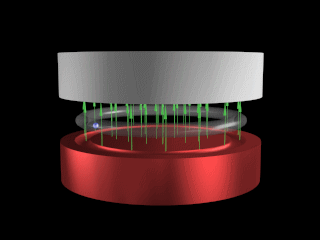
\includegraphics[width=0.5\textwidth]{Chp9_illus1.png}	
	\caption{练习12\quad 示意图}
\end{figure}
如图1,电子逆时针运动(俯视),其磁矩方向向下,故填“相反”。

\exercise{13}$BIR$\quad 垂直于纸面向里

\solve
$F=\int ||I\di{l}\times B||$。在这里可以将该电流投影到垂直于$B$的方向上,等效为从a指向圆心的电流。投影长度为$R$,故安培力大小为$BIR$,方向用等效的电流判断即可。

\exercise{14}$0.226\textrm{T}$\quad 300\ \textrm{A/m}

\solve
“细环”指细螺绕环,内部磁感应强度可看做处处相等。由安培环路定理:
\begin{gather*}
	H\cdot C=nI\\
	H=\dfrac{nI}{C}=300\ \textrm{A/m}
\end{gather*}
即先算出第二空。那么
\[
B=\mu_0\mu_rH=72\pi\times 10^{-3}\textrm{T}=0.226\textrm{T}
\]

\exercise{15}$5.36\times 10^{-3}\textrm{kg}\cdot \textrm{m}^2/\textrm{s}^2$

\solve
由题,沿y轴方向的导线固定,故它以及垂直于y轴的导线受的力矩均不影响线圈的运动。设边长为a,转动轴在y轴上,剩下一根导线受的力沿x轴负方向,则力矩为
\begin{align*}
	M&=Fa\sin \ang{40}\\
	&=BIa^2\sin \ang{40}\\
	&=7.2\sin \ang{40}\times 10^{-3}=5.36\times 10^{-3}
\end{align*}
保持位置不变,需要一等大反向的力矩。

\exercise{16}$2.3\times 10^{-5}$\quad 顺
 
\solve
参见练习8。

\exercise{17}0.5T\quad y轴正方向

\solve
由受力情况2得,磁场沿y轴,与情况1中“z轴正方向”垂直,故$M=m\times B=mB$,$B=
\dfrac{M}{m}=0.5\textrm{T}$。

由情况1及$M=m\times B$也易判断$B$的方向。

\exercise{18}逆时针方向

\solve
若无安培力,圆柱体在重力作用下有沿斜面向下滚动的趋势,所以其力矩方向为垂直于纸面向里。
为使安培力力矩垂直于纸面向外,可知磁矩方向是垂直于斜面向上的,于是可判断电流方向。

或者使用安培力的左手定则亦可:需要使左侧的电流受力向左而右侧的向右,使圆柱体有上滚的趋势。

\exercise{19}0.402 A

\solve
可以参考课本(黑皮)上册\rm{P}422例9.19。
\begin{figure}[!h]	
	\centering	
	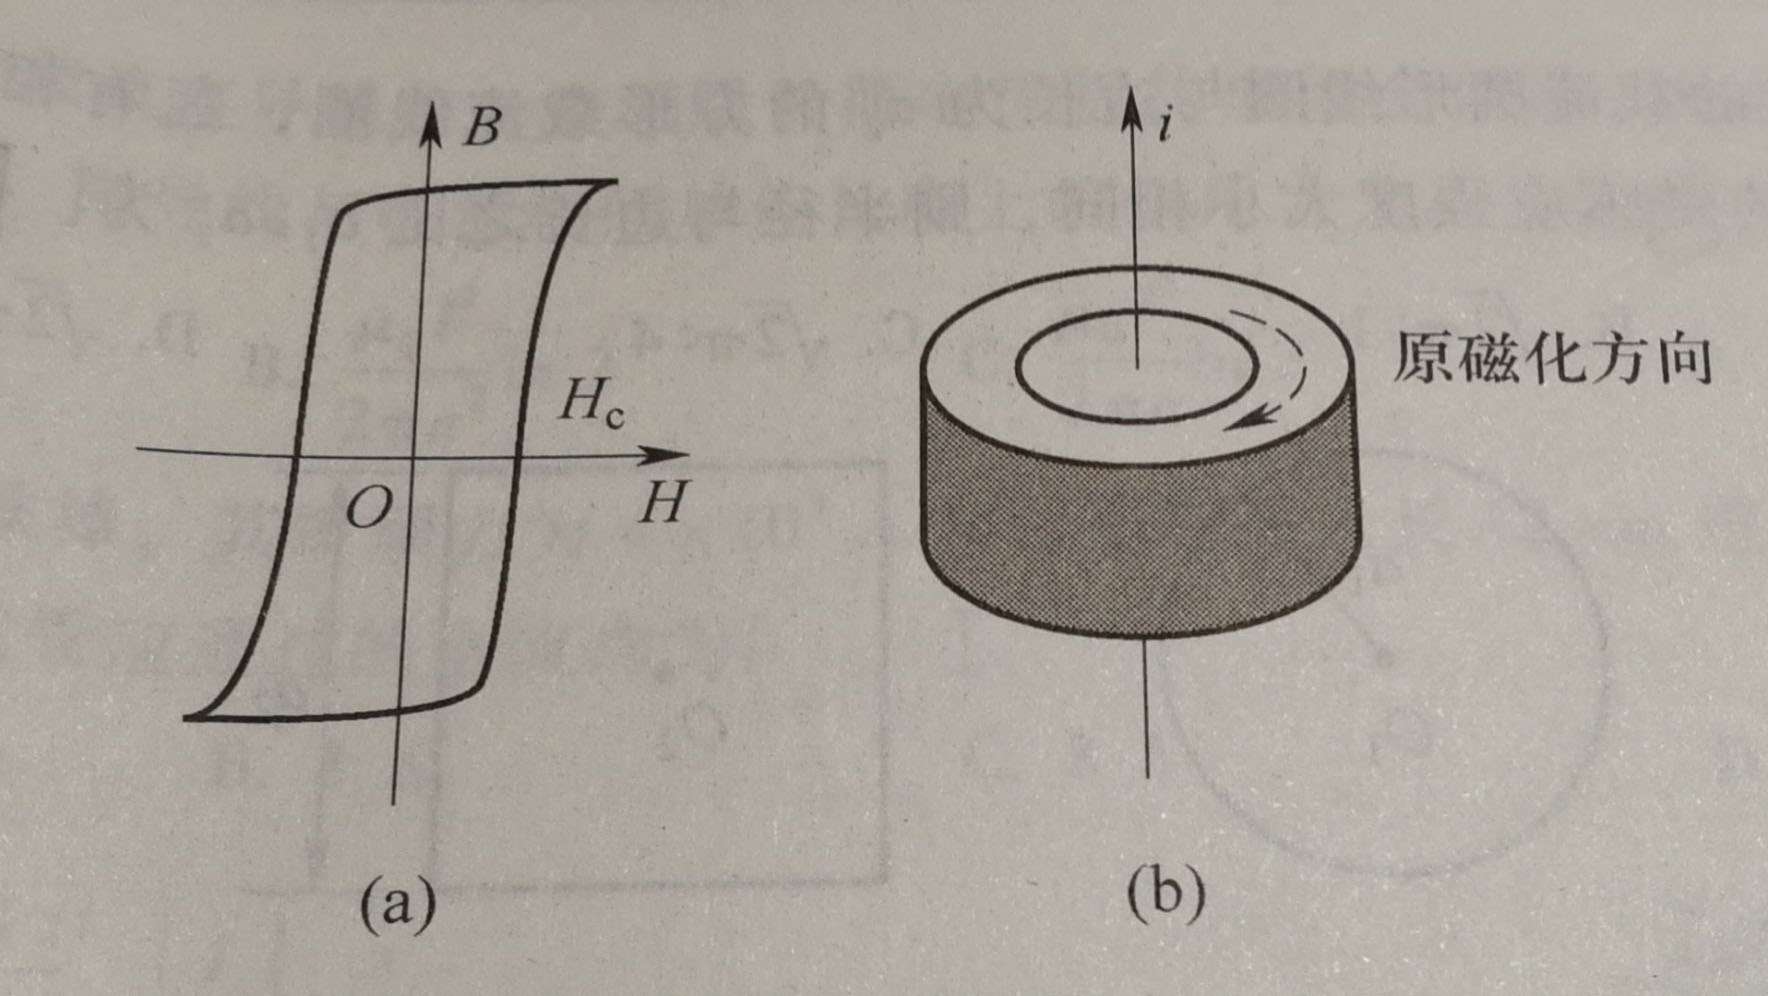
\includegraphics[width=0.5\textwidth]{Chp9_illus2.jpg}	
	\caption{练习12\quad 示意图}
\end{figure}

根据其磁滞回线,磁化后的磁芯处于曲线与B轴交点处。由题意,外加磁场强度大小等于矫顽力。而由安培环路定理,$H=\dfrac{i}{2\pi r}$,半径越大,磁场强度越小。要使磁芯的磁化方向完全翻转,需要有:
\begin{gather*}
	H_{R_2max}=\dfrac{i_{max}}{2\pi R_2}\geqslant H_c\\
	i_{max}\geqslant 2\pi R_2H_c=2\pi\cdot \dfrac{0.8\textrm{mm}}{2} \cdot 160\textrm{A/m}=0.402\textrm{A}
\end{gather*}
注意题中给的是直径。

\exercise{20}居里点(居里温度)

\solve
见课本铁磁质部分。

\section{解答题}

\exercise{21}

\solve
由题,板间磁场水平向右,可取如题图所示的回路,其上方的水平部分(标箭头的部分)位于板间的任意位置,且只有在这段回路上磁场环量不为零。由安培环路定理,$Hl=\sigma l$,则
$H=\sigma=1000 \textrm{A/m}\footnotemark[3]$
\footnotetext[3]
{可以作为结论来记忆。真空中平行板电容器的电场亦有$D=\sigma$(电荷面密度)}

由$B,H,M$三者的关系得:
\begin{align*}
		B&=\mu_0\mu_rH\\
		&=4\pi\times 10^{-7}\times 500\times 1000 \textrm{T}\\
		&=\dfrac{\pi}{5} \textrm{T}\\	
		M&=\dfrac{B}{\mu_0}-H\\
		&=(\mu_r-1)H\\
		&=4.99\times 10^5 \textrm{A/m}
\end{align*}

\exercise{22}

\solve
由于各段导线为直线,写出其矢量式,利用安培力公式即可\footnotemark[4]。
\footnotetext[4]{题中已建系或自己建系时,可以用$\vec{i},\vec{j},\vec{k}$表示方向,也可以再用“x轴正向”等描述。}
\begin{gather*}
	\vec{B}=0.6\vec{i}(\textrm{T})\\
	F_{ab}=I\cdot 0.6\vec{j}\times 0.6\vec{i}=-1.44\vec{k}(N)\\
	F_{bc}=I\cdot (0.6\vec{i}-0.6\vec{k})\times 0.6\vec{i}=-1.44\vec{j}(N)\\
	F_{cd}=I\cdot (0.6\vec{k}-0.6\vec{j})\times 0.6\vec{i}=1.44(\vec{j}+\vec{k})(N)\\
	F_{de}=I\cdot (-0.6\vec{k})\times 0.6\vec{i}=-1.44\vec{j}(N)\\
	F_{ef}=I\cdot (-0.6\vec{i})\times 0.6\vec{i}=0
\end{gather*}

\exercise{23}

\solve
(1)由安培环路定理,可知距AB为r处的磁感应强度$B=\dfrac{\mu_0I_1}{2\pi r}$

以D为原点,DN、DC为x、z轴建立空间直角坐标系。

对CD:
\begin{gather*}
	\vec{B}=\dfrac{\mu_0I_1}{2\pi d}\vec{j}\\
	F_{CD}=I_2\cdot b\vec{k}\times \vec{B}=-\dfrac{\mu_0I_1I_2b}{2\pi d}\vec{i}
\end{gather*}

对MN:
\begin{gather*}
	\vec{B}=\dfrac{\mu_0I_1}{2\pi (d+a)}\vec{j}\\
	F_{MN}=I_2\cdot b(-\vec{k})\times \vec{B}=\dfrac{\mu_0I_1I_2b}{2\pi (d+a)}\vec{i}
\end{gather*}

对CM:
\[
\vec{B}=\dfrac{\mu_0I_1}{2\pi (d+x)}\vec{j}
\]
\begin{align*}
	F_{CM}&=\int_{0}^{a}I_2\di{x}\cdot\vec{i}\times \vec{B}\\
	&=\dfrac{\mu_0I_1I_2}{2\pi}\vec{k}\int_{0}^{a}\dfrac{\di{x}}{x+d}\\
	&=\dfrac{\mu_0I_1I_2}{2\pi}\ln\dfrac{a+d}{d}\vec{k}
\end{align*}

对DN:
\[
\vec{B}=\dfrac{\mu_0I_1}{2\pi (d+x)}\vec{j}
\]
\begin{align*}
	F_{DN}&=\int_{0}^{a}I_2\di{x}\cdot(-\vec{i})\times \vec{B}\\
	&=-\dfrac{\mu_0I_1I_2}{2\pi}\vec{k}\int_{0}^{a}\dfrac{\di{x}}{x+d}\\
	&=-\dfrac{\mu_0I_1I_2}{2\pi}\ln\dfrac{a+d}{d}\vec{k}
\end{align*}
(2)
\begin{align*}
	F_\text{合}&=F_{CD}+F_{MN}+F_{CM}+F_{DN}\\
	&=\dfrac{\mu_0I_1I_2b}{2\pi}(\dfrac{1}{d+a}-\dfrac{1}{d})\vec{i}\\
	&=-\dfrac{\mu_0I_1I_2b}{2\pi d(d+a)}\vec{i}
\end{align*}

而$\vec{m},\vec{B}$均沿y轴正向,故$M=m\times B=0$
\footnotemark[5]。
\footnotetext[5]{对边受力不仅平行而且共线,线圈无转动趋势,所以力矩为零,不用考虑力矩是对哪个轴或点。}

\exercise{24}

\solve
电流密度$i=\dfrac{I}{\pi R^2-\pi r^2}$。
该系统可看作半径为$R$、电流密度为$i$的无限长圆柱面与半径为$r$、电流密度为$-i$的无限长圆柱面的组合。

由安培环路定理和磁感应强度叠加原理(向下为正向):
\begin{gather*}
	B_1\cdot 2\pi\cdot 2R=\mu_0i\cdot\pi R^2\\
	B_2\cdot 2\pi\cdot (2R+d)=-\mu_0i\cdot\pi r^2\\
	B_Q=B_1+B_2=\dfrac{\mu_0iR}{4}-\dfrac{\mu_0ir^2}{2(2R+d)}=\dfrac{\mu_0i}{2}(\dfrac{R}{2}-\dfrac{r^2}{2R+d})
\end{gather*}
由题图,$R>d>r$,故$B_Q$方向向下。
\[
F=e||v\times B_Q||=evB_Q=\dfrac{\mu_0Iev}{2\pi(R^2-r^2)}(\dfrac{R}{2}-\dfrac{r^2}{2R+d})
\]
由左手定则,$F$方向水平向左(沿OQ方向)。

\end{document}
